\documentclass{beamer}
\usetheme{Madrid}
\usepackage[utf8]{inputenc}
\usepackage[T1]{fontenc}
\usepackage{graphicx}
\usepackage{booktabs}
\usepackage{xcolor}
\usepackage{tikz}
\usetikzlibrary{shapes.geometric, arrows.meta, positioning, calc, patterns, decorations.pathreplacing}

% Professional dark teal/navy color scheme
\definecolor{primaryDark}{RGB}{0, 63, 92}
\definecolor{primaryMid}{RGB}{0, 95, 115}
\definecolor{accentGold}{RGB}{255, 190, 11}
\definecolor{lightBg}{RGB}{240, 244, 248}

\setbeamercolor{palette primary}{bg=primaryDark, fg=white}
\setbeamercolor{palette secondary}{bg=primaryMid, fg=white}
\setbeamercolor{palette tertiary}{bg=primaryDark, fg=white}
\setbeamercolor{palette quaternary}{bg=primaryDark, fg=white}
\setbeamercolor{structure}{fg=primaryDark}
\setbeamercolor{title}{fg=white, bg=primaryDark}
\setbeamercolor{frametitle}{fg=white, bg=primaryDark}
\setbeamercolor{block title}{bg=primaryMid, fg=white}
\setbeamercolor{block body}{bg=lightBg, fg=black}
\setbeamercolor{item}{fg=primaryMid}
\setbeamercolor{subitem}{fg=primaryMid}
\setbeamercolor{enumerate item}{fg=primaryDark}
\setbeamercolor{section in toc}{fg=primaryDark}
\title[MEMRES]{MEMRES: Memory-Augmented Agentic Python Dependency Resolver}
\author[Tran et al.]{
  {\small
  \textsuperscript{*}Tran Chi Nguyen,\quad
  \textsuperscript{*}Dao Sy Duy Minh,\quad
  \textsuperscript{*}Huynh Trung Kiet}\\[3pt]
  {\small
  Pham Phu Hoa,\quad
  Nguyen Lam Phu Quy}\\[6pt]
  {\scriptsize
  \{23122044, 23122041, 23122039, 23122030, 23122048\}@student.hcmus.edu.vn}
}
\institute[VNU-HCM]{University of Science, VNU-HCM\\[2pt]}
\date{FSE-AIWare 2026}

\begin{document}

\begin{frame}
  \titlepage
\end{frame}

% Motivation
\begin{frame}{Motivation}
  \begin{columns}[T]
  \begin{column}{0.55\textwidth}
  \begin{itemize}
    \item Python has 500,000+ PyPI packages --- dependency conflicts are pervasive.
    \item Legacy snippets frequently fail with ImportError, SyntaxError, version mismatch.
    \item PLLM (baseline): only 54.7\% success rate on HG2.9K.
    \item Need an agentic, memory-augmented approach that minimizes LLM reliance.
  \end{itemize}
  \end{column}
  \begin{column}{0.42\textwidth}
  \centering
  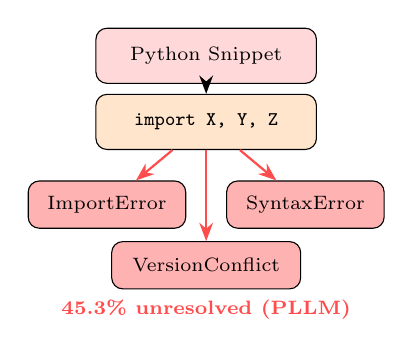
\begin{tikzpicture}[scale=0.7, every node/.style={font=\scriptsize}]
    % Problem illustration
    \node[draw, rounded corners, fill=red!15, minimum width=2.8cm, minimum height=0.7cm, align=center] (snippet) at (0,3) {Python Snippet};
    \node[draw, rounded corners, fill=orange!20, minimum width=2.8cm, minimum height=0.7cm, align=center] (imp) at (0,1.8) {\texttt{import X, Y, Z}};
    \node[draw, rounded corners, fill=red!30, minimum width=2cm, minimum height=0.6cm, align=center] (err1) at (-1.8,0.3) {ImportError};
    \node[draw, rounded corners, fill=red!30, minimum width=2cm, minimum height=0.6cm, align=center] (err2) at (1.8,0.3) {SyntaxError};
    \node[draw, rounded corners, fill=red!30, minimum width=2.4cm, minimum height=0.6cm, align=center] (err3) at (0,-0.8) {VersionConflict};
    \draw[-{Stealth}, thick] (snippet) -- (imp);
    \draw[-{Stealth}, thick, red!70] (imp) -- (err1);
    \draw[-{Stealth}, thick, red!70] (imp) -- (err2);
    \draw[-{Stealth}, thick, red!70] (imp) -- (err3);
    \node[font=\scriptsize\bfseries, text=red!70] at (0,-1.6) {45.3\% unresolved (PLLM)};
  \end{tikzpicture}
  \end{column}
  \end{columns}
\end{frame}

% Competition Overview
\begin{frame}{FSE-AIWare 2026 Competition}
  \begin{center}
  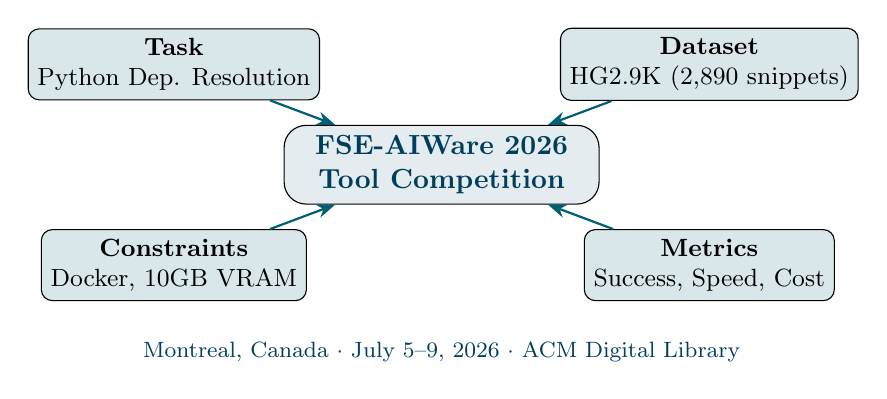
\begin{tikzpicture}[scale=0.85, every node/.style={font=\small}]
    % Central box
    \node[draw, rounded corners=8pt, fill=primaryDark!10, minimum width=4cm, minimum height=1cm, align=center, font=\normalsize\bfseries, text=primaryDark] (comp) at (0,0) {FSE-AIWare 2026\\Tool Competition};
    % Surrounding elements
    \node[draw, rounded corners, fill=primaryMid!15, minimum width=3cm, minimum height=0.8cm, align=center] (task) at (-4, 1.5) {\textbf{Task}\\Python Dep. Resolution};
    \node[draw, rounded corners, fill=primaryMid!15, minimum width=3cm, minimum height=0.8cm, align=center] (data) at (4, 1.5) {\textbf{Dataset}\\HG2.9K (2,890 snippets)};
    \node[draw, rounded corners, fill=primaryMid!15, minimum width=3cm, minimum height=0.8cm, align=center] (cons) at (-4, -1.5) {\textbf{Constraints}\\Docker, 10GB VRAM};
    \node[draw, rounded corners, fill=primaryMid!15, minimum width=3cm, minimum height=0.8cm, align=center] (met) at (4, -1.5) {\textbf{Metrics}\\Success, Speed, Cost};
    % Arrows
    \draw[-{Stealth}, thick, primaryMid] (task) -- (comp);
    \draw[-{Stealth}, thick, primaryMid] (data) -- (comp);
    \draw[-{Stealth}, thick, primaryMid] (cons) -- (comp);
    \draw[-{Stealth}, thick, primaryMid] (met) -- (comp);
    % Bottom note
    \node[font=\footnotesize, text=primaryDark] at (0, -2.8) {Montreal, Canada $\cdot$ July 5--9, 2026 $\cdot$ ACM Digital Library};
  \end{tikzpicture}
  \end{center}
\end{frame}

% System Architecture
\begin{frame}{MEMRES System Architecture}
  \begin{figure}
    
\includegraphics[width=0.9\linewidth]{pipeline.pdf}
    \caption{4-stage pipeline: Hybrid Evaluation, Module Cleaning, Version Selection, Build Loop}
  \end{figure}
  \begin{itemize}
    \item Multi-level confidence cascade: deterministic first, LLM as last resort.
    \item Memory-augmented: reuse proven solutions within the batch.
    \item Error Pattern KB: 200+ import $\rightarrow$ package mappings.
    \item Semantic Import Analyzer, Python 2 detector, system dependency injection.
  \end{itemize}
\end{frame}

% Confidence Cascade
\begin{frame}{Confidence Cascade}
  \begin{center}
  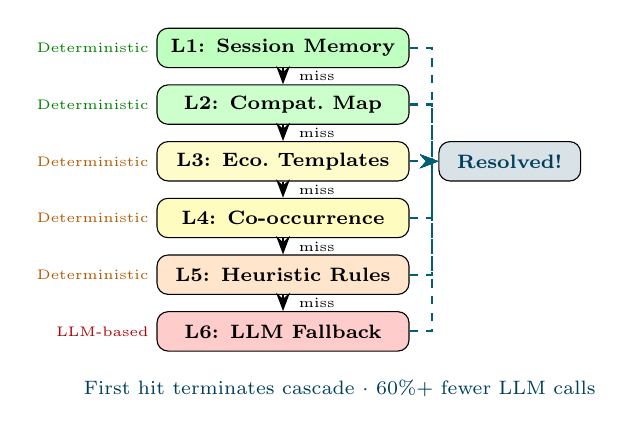
\begin{tikzpicture}[scale=0.72, every node/.style={font=\scriptsize},
    level/.style={draw, rounded corners=4pt, minimum width=3.2cm, minimum height=0.5cm, align=center, font=\scriptsize\bfseries}]
    % Levels - vertical flow
    \node[level, fill=green!25] (l1) at (0, 4.5) {L1: Session Memory};
    \node[level, fill=green!20] (l2) at (0, 3.5) {L2: Compat.\ Map};
    \node[level, fill=yellow!20] (l3) at (0, 2.5) {L3: Eco.\ Templates};
    \node[level, fill=yellow!25] (l4) at (0, 1.5) {L4: Co-occurrence};
    \node[level, fill=orange!20] (l5) at (0, 0.5) {L5: Heuristic Rules};
    \node[level, fill=red!20] (l6) at (0, -0.5) {L6: LLM Fallback};
    % Arrows
    \draw[-{Stealth}, thick] (l1) -- (l2) node[midway, right=2pt, font=\tiny] {miss};
    \draw[-{Stealth}, thick] (l2) -- (l3) node[midway, right=2pt, font=\tiny] {miss};
    \draw[-{Stealth}, thick] (l3) -- (l4) node[midway, right=2pt, font=\tiny] {miss};
    \draw[-{Stealth}, thick] (l4) -- (l5) node[midway, right=2pt, font=\tiny] {miss};
    \draw[-{Stealth}, thick] (l5) -- (l6) node[midway, right=2pt, font=\tiny] {miss};
    % Hit arrows
    \node[draw, rounded corners, fill=primaryDark!15, minimum width=1.8cm, minimum height=0.5cm, font=\scriptsize\bfseries, text=primaryDark] (res) at (4, 2.5) {Resolved!};
    \foreach \l in {l1,l2,l3,l4,l5,l6}
      \draw[-{Stealth}, dashed, primaryMid, thick] (\l.east) -- ++(0.4,0) |- (res);
    % Labels
    \node[font=\tiny, text=green!50!black, anchor=east] at (-2.2, 4.5) {Deterministic};
    \node[font=\tiny, text=green!50!black, anchor=east] at (-2.2, 3.5) {Deterministic};
    \node[font=\tiny, text=orange!70!black, anchor=east] at (-2.2, 2.5) {Deterministic};
    \node[font=\tiny, text=orange!70!black, anchor=east] at (-2.2, 1.5) {Deterministic};
    \node[font=\tiny, text=orange!70!black, anchor=east] at (-2.2, 0.5) {Deterministic};
    \node[font=\tiny, text=red!70!black, anchor=east] at (-2.2, -0.5) {LLM-based};
    % Summary
    \node[font=\scriptsize, text=primaryDark, align=center] at (1, -1.5) {First hit terminates cascade $\cdot$ 60\%+ fewer LLM calls};
  \end{tikzpicture}
  \end{center}
\end{frame}

% Key Techniques
\begin{frame}{Key Techniques}
  \begin{itemize}
    \item \textbf{Intra-Session Memory}: cache successful solutions for similar snippets.
    \item \textbf{Self-Evolving Memory}: learn tips/shortcuts via Jaccard similarity.
    \item \textbf{Error Pattern KB}: 200+ mappings, name corrections, version constraints, regex rules.
    \item \textbf{Semantic Analyzer}: analyze import usage patterns, detect ecosystems.
    \item \textbf{Python 2 Detector}: 13 indicators, automatic interpreter selection.
    \item \textbf{System Dependency Injection}: apt-get for C-extensions, version fallback cascade.
  \end{itemize}
\end{frame}

% Evaluation - Comparison
\begin{frame}{Evaluation: MEMRES vs.\ PLLM}
  \begin{columns}[T]
  \begin{column}{0.48\textwidth}
  \centering
  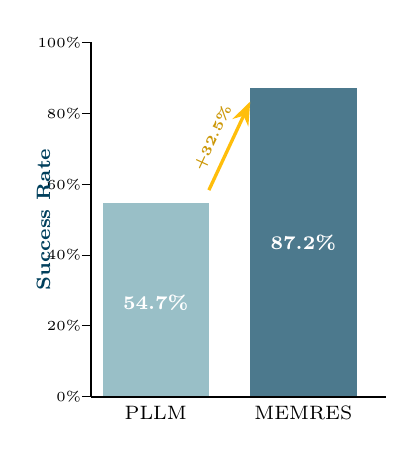
\begin{tikzpicture}[scale=0.75]
    % Bar chart
    \fill[primaryMid!40] (0,0) rectangle (1.8, 3.28); % PLLM 54.7%
    \fill[primaryDark!70] (2.5,0) rectangle (4.3, 5.23); % MEMRES 87.2%
    % Labels
    \node[font=\scriptsize\bfseries, text=white] at (0.9, 1.6) {54.7\%};
    \node[font=\scriptsize\bfseries, text=white] at (3.4, 2.6) {87.2\%};
    \node[font=\scriptsize, below] at (0.9, 0) {PLLM};
    \node[font=\scriptsize, below] at (3.4, 0) {MEMRES};
    % Axis
    \draw[thick] (-0.2,0) -- (4.8,0);
    \draw[thick] (-0.2,0) -- (-0.2,6);
    \foreach \y/\lbl in {0/0, 1.2/20, 2.4/40, 3.6/60, 4.8/80, 6.0/100}
      \draw (-0.35,\y) -- (-0.2,\y) node[left, font=\tiny] {\lbl\%};
    \node[font=\scriptsize\bfseries, text=primaryDark, rotate=90] at (-1.0, 3) {Success Rate};
    % Delta arrow
    \draw[-{Stealth}, very thick, accentGold] (1.8, 3.5) -- (2.5, 5.0) node[midway, above, font=\tiny\bfseries, text=accentGold!80!black, sloped] {+32.5\%};
  \end{tikzpicture}
  \end{column}
  \begin{column}{0.50\textwidth}
  \small
  \begin{tabular}{lrr}
    \toprule
    \textbf{Metric} & \textbf{PLLM} & \textbf{MEMRES} \\
    \midrule
    Resolved & 1,583 & \textbf{2,519} \\
    Failed & 1,308 & \textbf{371} \\
    Success & 54.7\% & \textbf{87.2\%} \\
    \bottomrule
  \end{tabular}
  \vspace{0.5em}
  \begin{itemize}\itemsep2pt
    \item[\textcolor{primaryDark}{$\bullet$}] Setup: HG2.9K, Gemma-2 9B, Docker
    \item[\textcolor{primaryDark}{$\bullet$}] 950+ PLLM failures resolved
    \item[\textcolor{primaryDark}{$\bullet$}] 53.9\% needed sys-dep classifiers
  \end{itemize}
  \end{column}
  \end{columns}
\end{frame}

% Evaluation - Ablation
\begin{frame}{Ablation Study: Resolution by Component}
  \begin{center}
  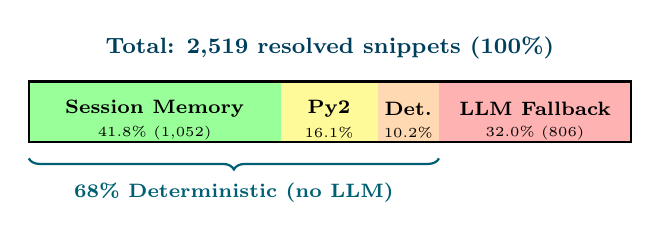
\begin{tikzpicture}[scale=0.85]
    % Stacked horizontal bar
    \def\totalW{9}
    \def\barH{0.9}
    % Session Memory 41.8%
    \fill[green!40] (0,0) rectangle ({0.418*\totalW}, \barH);
    \node[font=\scriptsize\bfseries, text=black] at ({0.209*\totalW}, {0.55*\barH}) {Session Memory};
    \node[font=\tiny] at ({0.209*\totalW}, {0.15*\barH}) {41.8\% (1,052)};
    % Python 2 Heuristic 16.1%
    \fill[yellow!40] ({0.418*\totalW},0) rectangle ({0.579*\totalW}, \barH);
    \node[font=\scriptsize\bfseries, text=black] at ({0.4985*\totalW}, {0.55*\barH}) {Py2};
    \node[font=\tiny] at ({0.4985*\totalW}, {0.15*\barH}) {16.1\%};
    % Deterministic L2-5 10.2%
    \fill[orange!30] ({0.579*\totalW},0) rectangle ({0.681*\totalW}, \barH);
    \node[font=\scriptsize\bfseries, text=black] at ({0.630*\totalW}, {0.55*\barH}) {Det.};
    \node[font=\tiny] at ({0.630*\totalW}, {0.15*\barH}) {10.2\%};
    % LLM Fallback 32.0%
    \fill[red!30] ({0.681*\totalW},0) rectangle ({\totalW}, \barH);
    \node[font=\scriptsize\bfseries, text=black] at ({0.8405*\totalW}, {0.55*\barH}) {LLM Fallback};
    \node[font=\tiny] at ({0.8405*\totalW}, {0.15*\barH}) {32.0\% (806)};
    % Border
    \draw[thick] (0,0) rectangle ({\totalW}, \barH);
    % Legend
    \node[font=\footnotesize\bfseries, text=primaryDark] at ({\totalW/2}, {\barH+0.5}) {Total: 2,519 resolved snippets (100\%)};
    % Brace for deterministic
    \draw[decorate, decoration={brace, amplitude=4pt, mirror}, thick, primaryMid] (0,-0.25) -- ({0.681*\totalW},-0.25) node[midway, below=5pt, font=\scriptsize\bfseries, text=primaryMid] {68\% Deterministic (no LLM)};
  \end{tikzpicture}
  \end{center}
  \vspace{-0.3em}
  \begin{itemize}\small
    \item 68\% of resolutions require \textbf{zero LLM calls}.
    \item Session Memory alone handles 41.8\% via proven cached solutions.
    \item Python 2 detector resolves the single largest failure category from PLLM.
  \end{itemize}
\end{frame}

% Failure Analysis
\begin{frame}{Failure Analysis (371 failures)}
  \begin{center}
  \begin{tabular}{llrr}
    \toprule
    \textbf{Category} & \textbf{Root Cause} & \textbf{Count} & \textbf{\%} \\
    \midrule
    Build / C-ext & Missing C toolchains, heavy packages & 186 & 50.1\% \\
    ImportError & Obscure/deprecated packages & 121 & 32.6\% \\
    Timeout & Large ML package compilation & 55 & 14.8\% \\
    System/Platform & GTK, RPi, platform-specific & 9 & 2.4\% \\
    \midrule
    \textbf{Total} & & \textbf{371} & \textbf{100\%} \\
    \bottomrule
  \end{tabular}
  \end{center}
  \vspace{0.5em}
  \begin{itemize}\small
    \item Most failures are \textbf{inherently unresolvable} in Docker (no C toolchain, no GPU).
    \item 32.6\% from packages completely absent from PyPI (deprecated/renamed).
    \item Only 2.4\% are platform-specific (GTK, Raspberry Pi, Maya).
  \end{itemize}
\end{frame}

% Limitations & Lessons
\begin{frame}{Limitations \& Lessons Learned}
  \begin{itemize}
    \item Failures dominated by C-extension build errors, deprecated packages, timeouts.
    \item Session memory is order-sensitive, but deterministic cascade ensures accuracy.
    \item Runtime passes (system-only imports) are strictly counted as failures.
    \item Key insight: deterministic rules + memory augmentation outperform LLM-only.
  \end{itemize}
\end{frame}

% Conclusion
\begin{frame}{Conclusion}
  \begin{itemize}
    \item MEMRES: agentic resolver with memory augmentation and confidence cascade.
    \item Achieves 87.2\% success on HG2.9K, significantly surpassing PLLM (54.7\%).
    \item Reduces computational cost by minimizing LLM calls (60\%+ reduction).
    \item Contributions: novel pipeline, Error Pattern KB, self-evolving memory, Python 2 heuristics, system dependency injection.
  \end{itemize}
  \vspace{1em}
  \centering\textbf{Thank you!}
\end{frame}

\end{document}